\documentclass[12pt]{article}
\usepackage{enumerate}
\usepackage{notes}
\usepackage{oxford}

\begin{document}

\section{A0 - Linear Algebra}
\subsection{Basis of space of functions $f:\N \to \R$}
\red{Doesn't this suggest, contra the question, that every basis of $F_\infty$
  is countable? Let's attempt to prove that and see what goes wrong...
  ~\\\\
  Basic question: if I show it is true for all finite sets $1, 2, \ldots, n$,
  that is not the same as showing that it true for $\N$, right?
}

\hrule
~\\
Alternatively, do something like a diagonal argument: enumerate the elements of
a basis, and then show that there is an element of the basis that is not
contained within the enumeration.


\section{A1 - Differential Equations}
\subsection{Picard theorem}
\textbf{P(i)} (b) ?\\
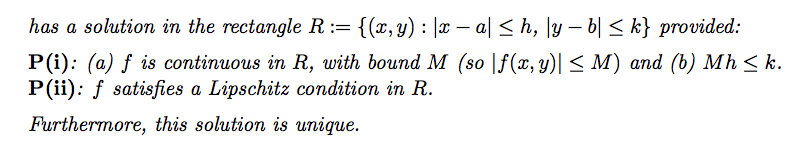
\includegraphics[width=400pt]{img/question-differential-equations-a1-picard.png}\\


\end{document}
